\svnidlong
{$HeadURL: $}
{$LastChangedDate: $}
{$LastChangedRevision: $}
{$LastChangedBy: $}
\svnid{$Id: $}   

% +++++++++++++++++++++++++++++++++++++++++++++++++++++++++++++++++++++++++++++++++++++
% Linda 11/5/2015
% +++++++++++++++++++++++++++++++++++++++++++++++++++++++++++++++++++++++++++++++++++++

%Despite the appearance of simplified models, we argue that
%the model independent approach of the EFTs is still relevant.
The EFT operators considered in this section do not have an implementation 
of a simplified model completion for Dirac fermion Dark Matter available to date. 
They provide kinematic distributions that 
are unique to mono-boson signatures, and that in most cases 
are not reproduced by an equivalent simplified model.\sidenote{Wherever this is
the case, for practical reasons one can only generation a simplified model result 
in the limiting EFT case, as the results can be rescaled and reinterpreted.}

A complete list of effective operators with direct DM/boson couplings for
Dirac DM, up to dimension 7, can be found in~\cite{Cotta:2012nj, Carpenter:2012rg, Crivellin:2015wva}. 
Higher dimensional operators, up to dimension 8, leading to Higgs+\MET signatures,
are mentioned in~\cite{Carpenter:2012rg, Berlin:2014cfa}. The first part of this Section outlines
the main characteristics for a limited number of these models that could be 
considered in early Run-2 searches. 
However, the EFT approximation made for these operators can be problematic, see Ref.~\cite{Berlin:2014cfa} for discussion.
For this reason, model-independent results as in Appendix~\ref{app:Presentation_Of_Experimental_Results} 
should be privileged over considering these operators as realistic benchmarks. 
%We also recommend not to optimize searches based on those benchmark models. 

However, the Forum discussion highlighted that the EFT approach allows
more model-independence when reinterpreting results, and that it is worth still considering
interpretation of the results available in terms of these operators. Furthermore, once simplified models are available
for those operators, EFT results can be used as a limiting case for consistency checks. 
We devote the end of this Section to a discussion on the presentation of results 
from this model, including an assessment of their reliability 
using a conservative procedure that is only dependent on EFT parameters.

The studies in this Section
have been performed using a UFO model within \madgraph v2.2.3, interfaced to \pythia 8 for the parton shower.  
The implementation of these models is discussed further in Section~\ref{sub:EFTModels}.

%CD: what is this?
%\newthought{Implementation discussed in the Appendix}

%%%%%%%%%%%Dimension 5 operators
\subsection{Dimension 5 operators}
\label{sub:EW_EFT_Dim5}

The lowest dimension benchmark operators we consider are effective dimension 5,
such as the one depicted in Figure~\ref{fig:modelMonoHEFT}.  

\begin{figure}[!htb]
	\centering
	\unitlength=0.005\textwidth
    \vspace{3\baselineskip}
	\begin{feynmandiagram}[modelMonoHEFT]
		\fmfleft{i1,i2}
		\fmfright{o1,o2,ohidden,o3}
		\fmf{fermion}{i2,v1,i1}
		\fmflabel{\Large $q,g$}{i2}
		\fmflabel{\Large $\bar{q},g$}{i1}
		\fmf{dashes}{v1,v2}
		\fmfv{decor.shape=circle,decor.filled=shaded, decor.size=30,label={\Large $\text{EFT}(\lambda,,\Lambda)$},label.a=30,label.d=15}{v2}
		\fmf{dashes}{v2,o3}
		\fmflabel{\Large $h$}{o3}
		\fmf{fermion}{o2,v2,o1}
		\fmflabel{\Large ${\bar{\chiDM}}$}{o1}
		\fmflabel{\Large ${\chiDM}$}{o2}
		\fmfdot{v1}
	\end{feynmandiagram}
    \vspace{3\baselineskip}
	\caption{Diagram for EFT operators giving rise to a Higgs+\MET signature.}
	\label{fig:modelMonoHEFT}
\end{figure}

Following the notation of~\cite{Carpenter:2012rg},  models
from this category have a Lagrangian that, after electroweak symmetry breaking, 
includes terms such as:

\begin{eqnarray}
\frac{m_W^2}{\Lambda_5^3} ~\bar{\chiDM} \chiDM ~W^{+ \mu} W^{-}_\mu
+ \frac{m_Z^2}{2 \Lambda_5^3} ~ \bar{\chiDM} \chiDM ~ Z^\mu Z_\mu ~,
\end{eqnarray}
where $m_Z$ and $m_W$ are the masses of the $Z$ and $W$ boson, $W^{\mu}$ and $Z^{\mu}$
are the fields of the gauge bosons, $\chiDM$ denotes the Dark Matter fields
and $\Lambda_5$ is the effective field theory scale. Note that these operators are of true dimension 7, 
but reduce to effective dimension 5 once the Higgs vacuum expectation values, 
contained in the W and Z mass terms, are inserted.  
As such, one expects that these operators would naturally arise in UV complete models where Dark Matter 
interacts via a Higgs portal where heavy mediators couple to the Higgs or other fields in an extended Higgs sector. 
In such models the full theory may be expected to contain additional operators with Higgs-Dark Matter couplings~\cite{Djouadi:2012zc}.
The above operator also induces signatures with 
\MET in conjunction with Z and W bosons at tree level, as shown in Fig.~\ref{fig:VPlusMET_EFT},
while at loop level it induces couplings to photon pairs and $Z \gamma$ through W loops.
In these models, a clear relation exists between final states with photons, EW bosons
and Higgs boson. 

As shown in Fig.~\ref{fig:EW_EFT5_Zlep_MET}, the 
kinematics of this model can be approximated by that of a simplified model including 
a high-mass scalar mediator exchanged in the \schannel described in Section~\ref{sub:EW_Scalar}. 
For this reason, the list of benchmark models with direct boson-DM couplings for photon, Z and W 
only includes dimension 7 operators: if the scalar model with initial state radiation of an EW boson
is already generated, then its results can be rescaled. 

The Higgs+\MET analysis,
however, will not consider the scalar simplified model as benchmark, due to the very low sensitivity 
in early LHC analyses, and will instead use this dimension 5 operator. 

\begin{figure}
	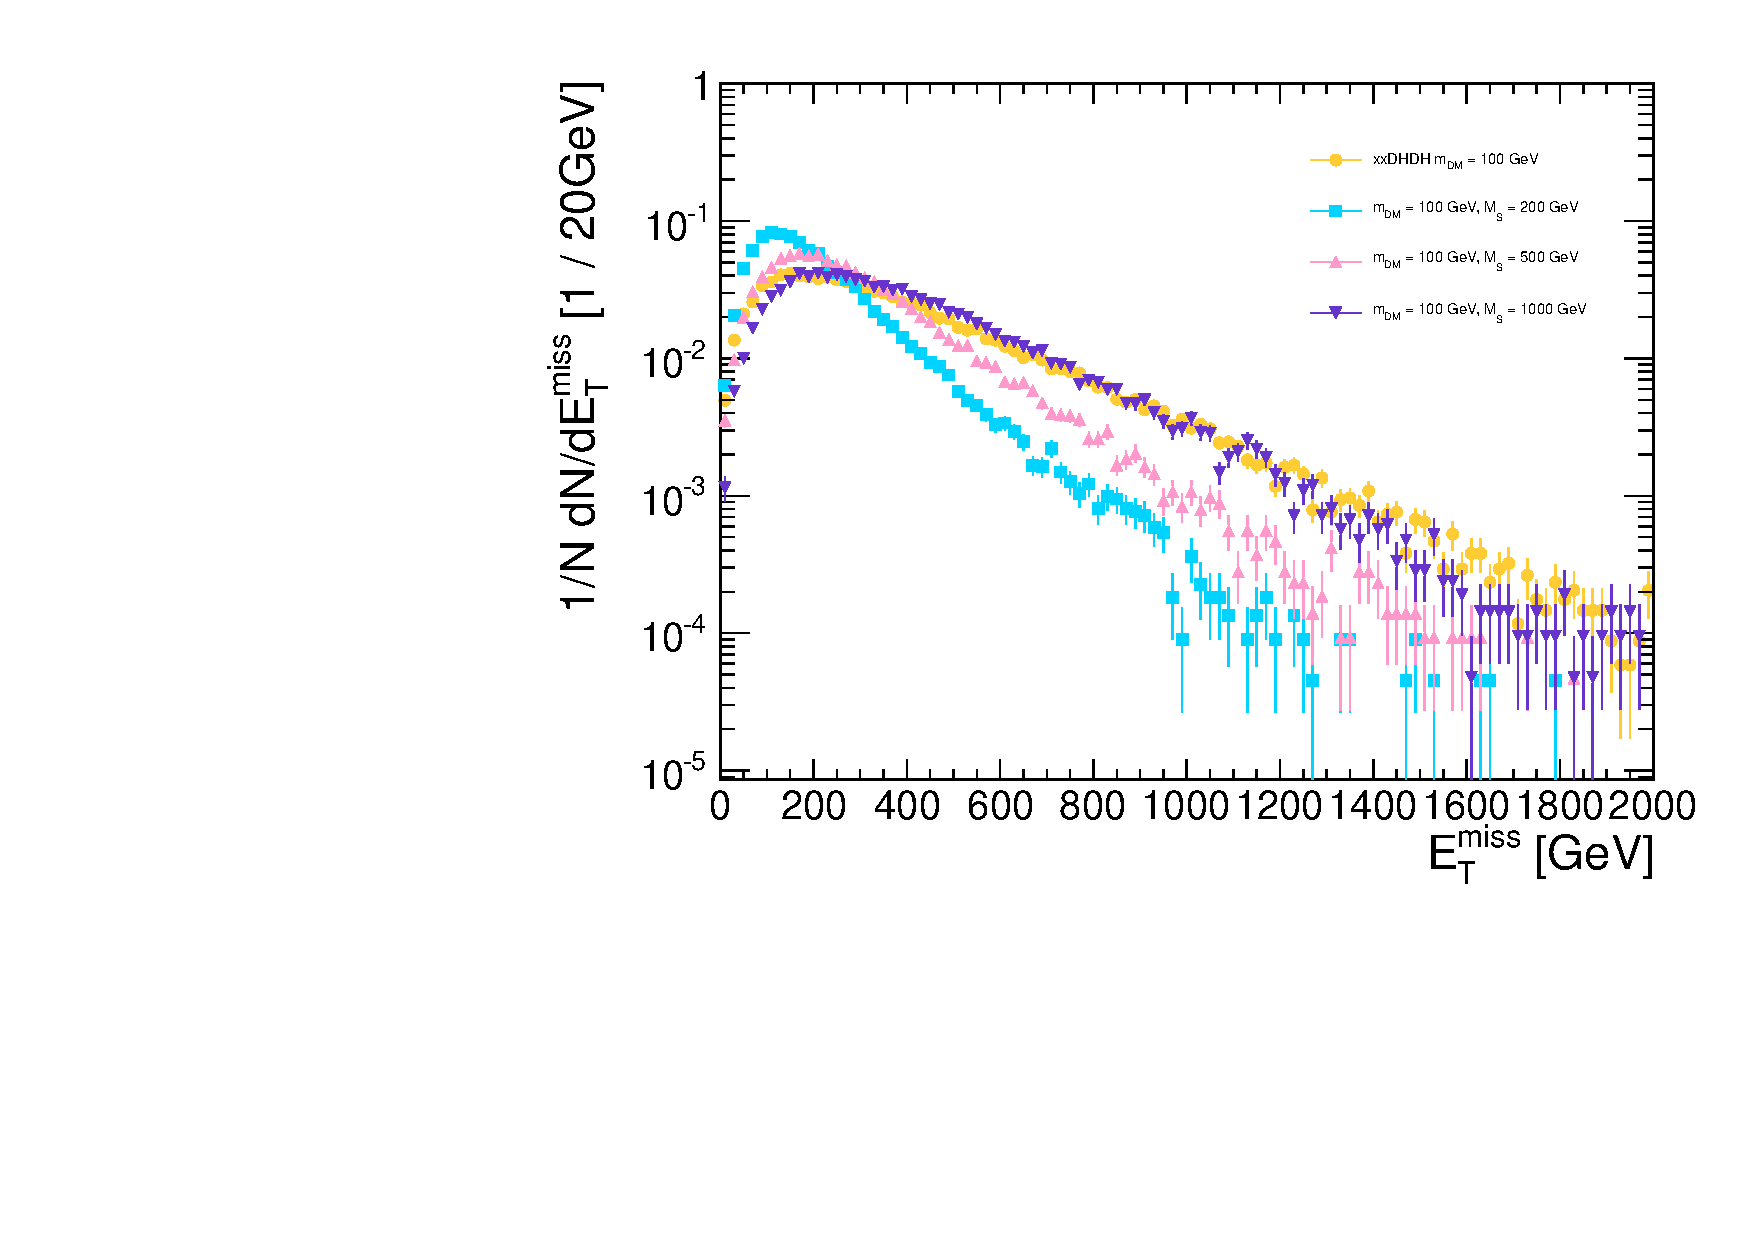
\includegraphics[width=0.95\textwidth]{figures/EW/pt_vv2_xxDHDH_vs_ScalarMediator.pdf}
	\caption{Comparison of the missing transverse momentum for the simplified model
		where a scalar mediator is exchanged in the \schannel and the model including 
		a dimension-5 scalar contact operator, in the leptonic Z+\MET final state. All figures in this Section
		have been performed using a UFO model within \madgraph v2.2.3, interfaced to \pythiaEight for the parton shower.  }
	\label{fig:EW_EFT5_Zlep_MET}
\end{figure}

\subsubsection{Parameter scan}

The two parameters of this model are the scale of new physics $\lambda$ 
and the DM particle mass. SM-DM coupling and new physics scale are related by 
$\gDM = {(246~\gev)}/{\lambda}$. 


The initial value of the new physics scale $\lambda$ chosen 
for the sample generation is 3~\tev. This is a convention and does not affect the signal kinematics:
the cross-section of the samples can be rescaled when deriving the constraints on this scale. 
However, more care should be given when rescaling Higgs+\MET operators
of higher dimensions, as different diagrams have a different $\lambda$ dependence. 
%From Andy
%– Lambda=3~\tev. Essentially this is an arbitrary choice for most EFTs, 
%however it does affect the mono-H analysis as some of their models 
%have non-trivial scaling with Λ. More care should be given to the choice for mono-H. 

The DM mass values for the benchmark points to be simulated are chosen to
span a sufficient range leading to different kinematics, 
that is within the LHC sensitivity for early searches and that is consistent across 
the various signatures and EFT operators. We therefore start the mass scan
at \mdm=1~\gev, where collider experiments are complementary to direct and indirect detection
and choose the last point corresponding to a DM mass of 1~\tev. 
We recommend a scan in seven mass points, namely:
$$
\mdm = { 1, 10, 50, 100, 200, 400, 800, 1300 } \gev. 	
$$

A set of kinematic distributions from the Higgs+\MET signature where the Higgs decays 
into two $b-$quarks is shown in Fig.~\ref{fig:Hbb_Dim5}, for points similar to those of the grid scan proposed. 
  
 \begin{figure}[hbpt!]
 	\centering
 	\subfloat[Leading $b-$jet transverse momentum]{
 		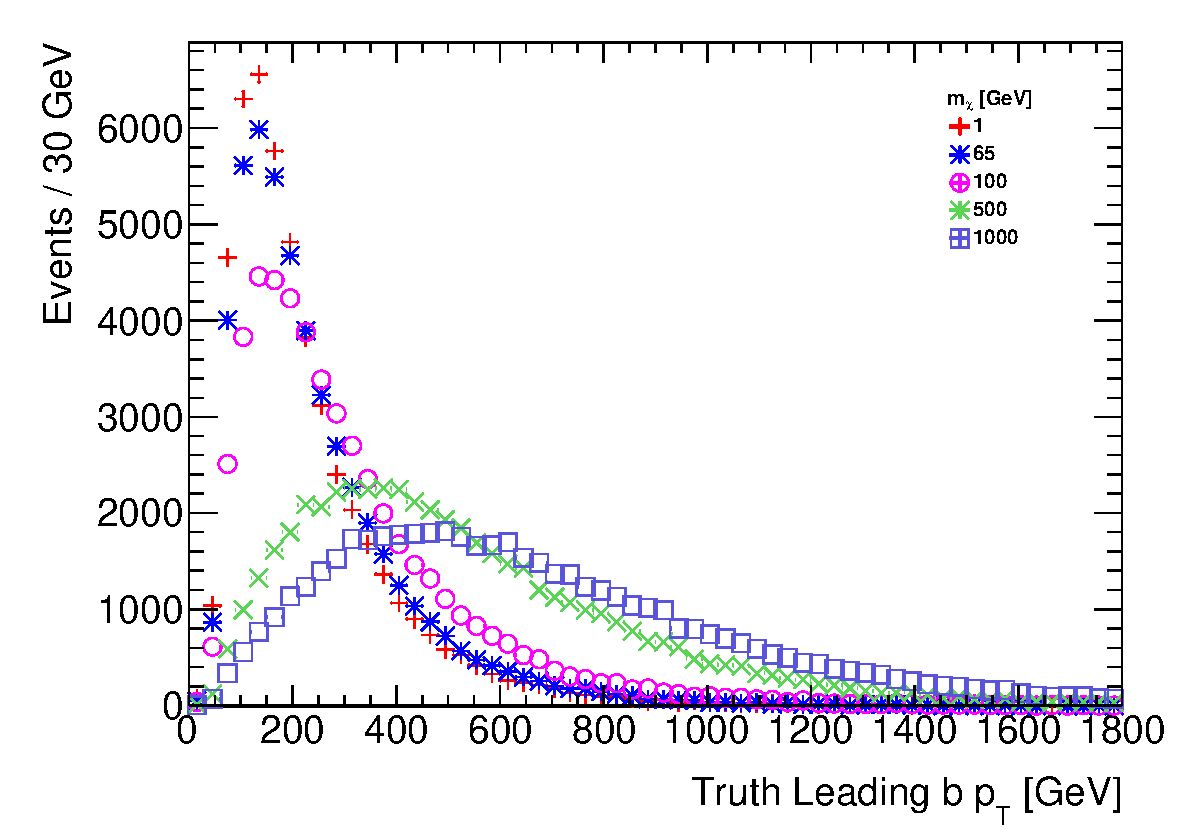
\includegraphics[width=0.8\linewidth]{figures/EW/monoH/xxhhg5/truth_leading_b_pt} %\label{fig:met_cmp_high}
 	}
 	\hfill
 	\subfloat[Leading $b-$jet pseudorapidity]{
 		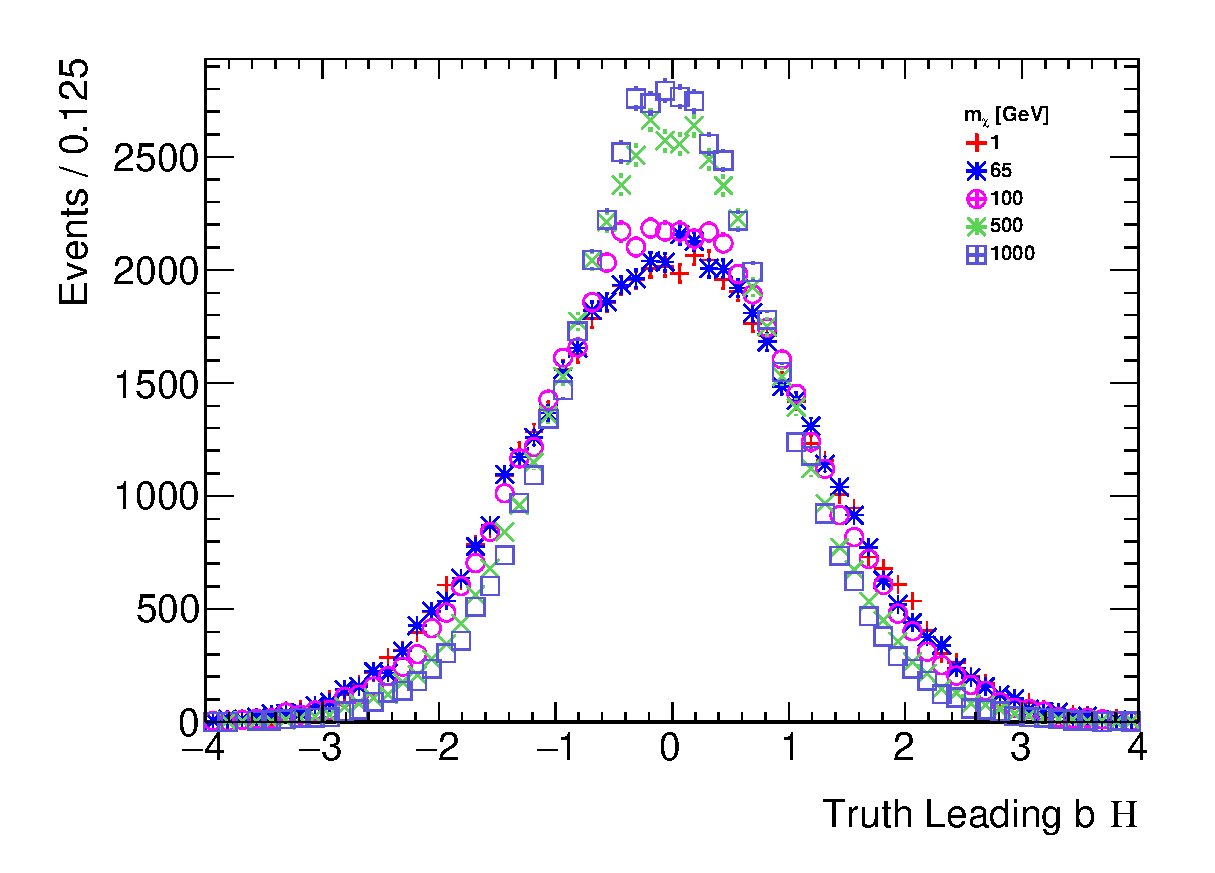
\includegraphics[width=0.8\linewidth]{figures/EW/monoH/xxhhg5/truth_leading_b_eta} %\label{fig:met_cmp_low}
 	}
 	\hfill
% 	\subfloat[Leading $b-$jet transverse momentum]{
% 		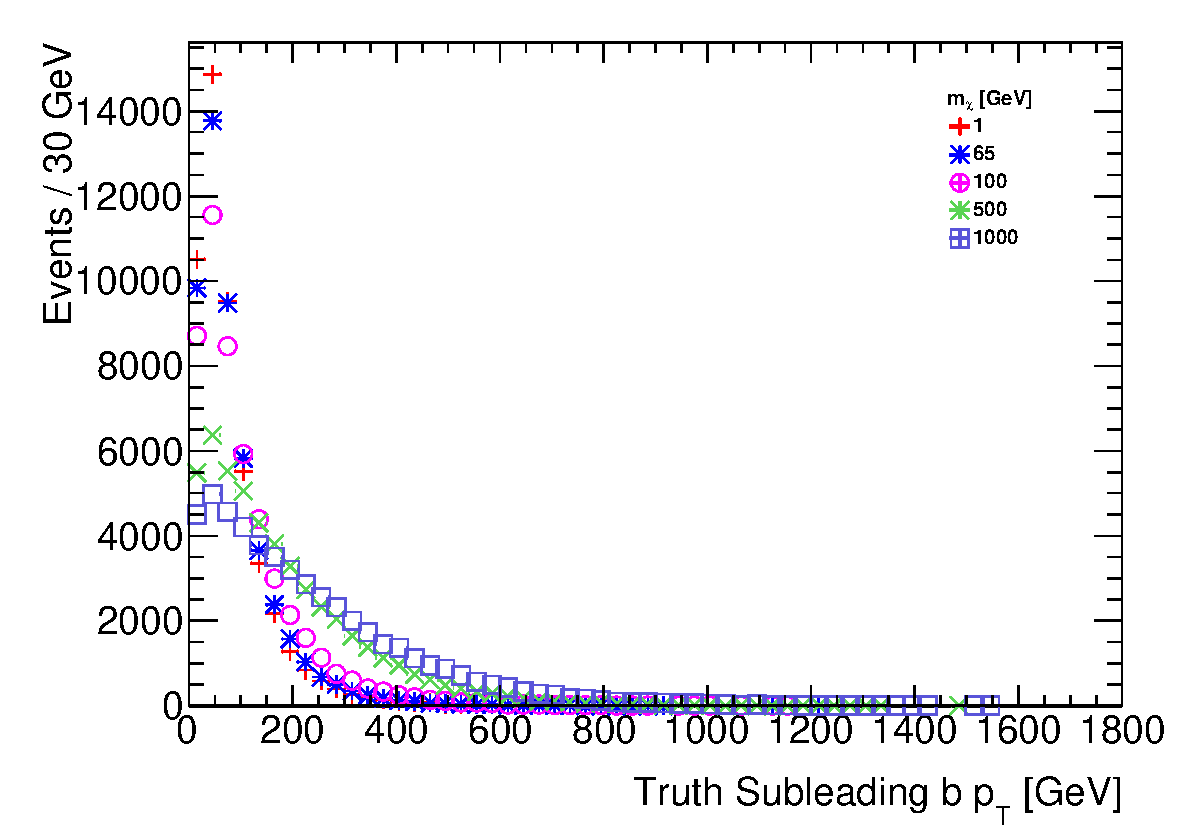
\includegraphics[width=0.95\linewidth]{figures/EW/monoH/xxhhg5/truth_subleading_b_pt} %\label{fig:met_cmp_high}
% 	}
% 	\hfill
% 	\subfloat[Leading $b-$jet pseudorapidity]{
% 		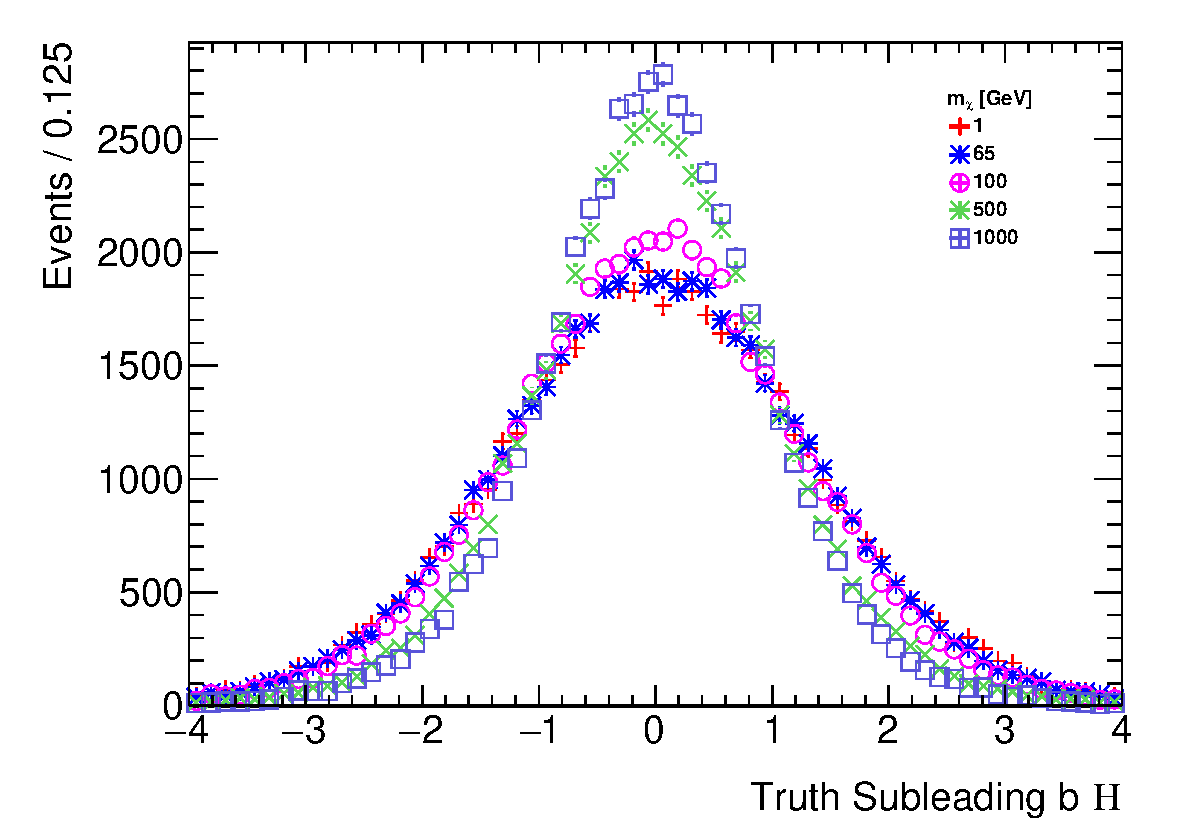
\includegraphics[width=0.95\linewidth]{figures/EW/monoH/xxhhg5/truth_subleading_b_eta} %\label{fig:met_cmp_low}
% 	}
% 	\hfill

 	\subfloat[Angular distance between the two leading $b-$jets]{
 		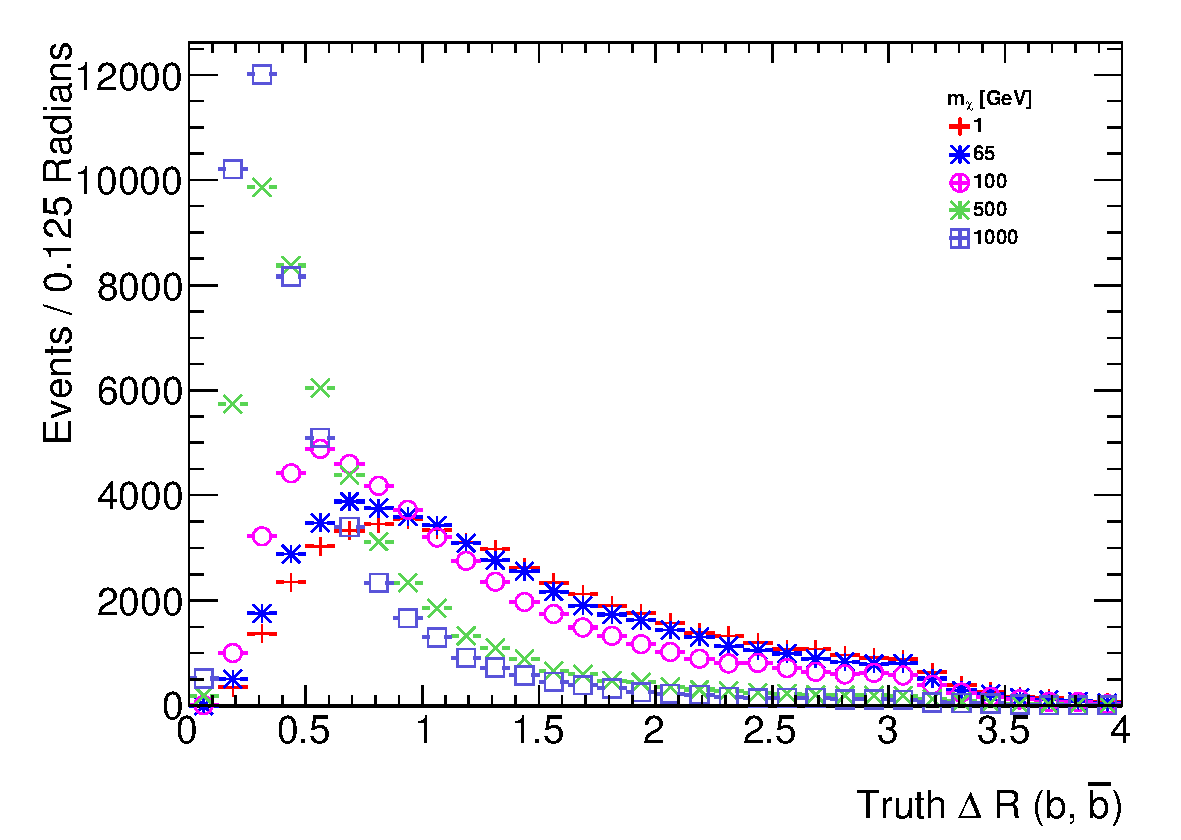
\includegraphics[width=0.8\linewidth]{figures/EW/monoH/xxhhg5/truth_bb_deltar} %\label{fig:met_cmp_low}
 	}
 	\caption{Comparison of the kinematic distributions for the two leading $b-$ jets (from the Higgs decay) in the model with direct interactions
 		between the Higgs boson and the DM particle, when varying the DM mass. 
 		\label{fig:Hbb_Dim5}}
 \end{figure}
 
 
%%%%%%%%%%%%%Dimension 7 operators

\subsection{Dimension 7 operators}
\label{sub:EW_EFT_Dim7}

% +++++++++++++++++++++++++++++++++++++++++++++++++++++++++++++++++++++++++++++++++++++
% Uli 3/5/2015
% +++++++++++++++++++++++++++++++++++++++++++++++++++++++++++++++++++++++++++++++++++++

The dimension-7 benchmark models  contain the $SU(2)_L \times U(1)_Y$ gauge-invariant couplings between 
DM fields and the kinetic terms of the EW bosons. The CP-conserving scalar couplings of this type can be written as
\begin{equation} \label{eq:Lc1c2}
\frac{c_1}{\Lambda_S^3} \, \bar \chiDM \chiDM \, B_{\mu \nu} B^{\mu \nu }  + \frac{c_2}{\Lambda_S^3} \, \bar \chiDM \chiDM \, W_{\mu \nu}^i W^{i, \mu \nu }  \,.
\end{equation}
Here $B_{\mu \nu} = \partial_\mu B_\nu - \partial_\nu B_\mu$ and $W_{\mu \nu}^i =  \partial_\mu W_\nu^i - \partial_\nu W_\mu^i + g_2 \hspace{0.25mm} \epsilon^{ijk}  \hspace{0.25mm}  W_\mu^j \hspace{0.25mm} W_\mu^k$ are the $U(1)_Y$ and $SU(2)_L$ field strength tensor, respectively, and  $g_2$ denotes the weak coupling constant. In the case of the pseudoscalar couplings, one has instead
\begin{equation} \label{eq:Lc3c4}
\frac{c_1}{\Lambda_P^3} \, \bar \chiDM \gamma_5 \chiDM \, B_{\mu \nu} \tilde B^{\mu \nu }  + \frac{c_2}{\Lambda_P^3} \, \bar \chiDM \gamma_5 \chiDM \, W_{\mu \nu}^i \tilde W^{i, \mu \nu }  \,,
\end{equation}
where $\tilde B_{\mu \nu} = 1/2 \hspace{0.5mm} \epsilon_{\mu \nu  \lambda \rho}  \hspace{0.25mm}  B^{\lambda \rho}$ and $\tilde W_{\mu \nu}^i = 1/2 \hspace{0.5mm} \epsilon_{\mu \nu  \lambda \rho}  \hspace{0.25mm}  W^{i, \lambda \rho}$ are the dual  field strength tensors. In addition to the CP-conserving interactions (\ref{eq:Lc1c2}) and (\ref{eq:Lc3c4}), there are also four CP-violating couplings that are obtained from the above operators by the replacement $\bar \chiDM \chiDM \leftrightarrow \bar \chiDM \gamma_5 \chiDM$.

The effective interactions introduced in (\ref{eq:Lc1c2}) and  (\ref{eq:Lc3c4}) appear  in models of Rayleigh DM~\cite{Weiner:2012cb}. Ultraviolet completions where the operators are generated through loops of states charged under $U(1)_Y$ and/or $SU(2)_L$  have been proposed in \cite{Weiner:2012gm} and their LHC signatures have been studied in \cite{Liu:2013gba}. If these new charged particles  are  light, the high-$p_T$ gauge bosons that participate in  the \MET processes considered here are able to resolve the substructure of the loops. This generically suppresses the cross sections compared to the EFT predictions~\cite{Haisch:2012kf}, and thus will weaken the bounds on the interaction strengths of  DM and the EW gauge bosons  to some extent.  Furthermore, the light charged mediators may be produced  on-shell in $pp$ collisions, rendering direct LHC searches potentially more restrictive than \MET searches. Making the above statements precise would require further studies beyond the timescale of this forum.

Since for $\Lambda_S = \Lambda_P$ the effective interactions (\ref{eq:Lc1c2}) and (\ref{eq:Lc3c4}) predict essentially the same value of the mono-photon, mono-$Z$ and mono-$W$ cross section \cite{Carpenter:2012rg,Crivellin:2015wva}, we consider below only the former couplings. We emphasize however that measurements of the jet-jet azimuthal angle difference in \MET$+ 2 j$ events may be used to disentangle whether DM couples more strongly to the combination $B_{\mu \nu} B^{\mu \nu}$ ($W_{\mu \nu}^i W^{i, \mu \nu }$) or the product $B_{\mu \nu} \tilde B^{\mu \nu}$ ($W_{\mu \nu}^i \tilde W^{i, \mu \nu }$) of field strength tensors \cite{Cotta:2012nj,Crivellin:2015wva}.

After EW symmetry breaking the interactions (\ref{eq:Lc1c2}) induce direct couplings 
between pairs of DM particles and  gauge bosons.  The corresponding Feynman rule reads:

\begin{equation}  \label{eq:feynman}
\frac{4 \hspace{0.25mm} i}{\Lambda_S^3} \; g_{V_1 V_2} \, \big (  p_1^{\mu_2} \hspace{0.25mm} p_2^{\mu_1} - g^{\mu_1 \mu_2}  \, p_1 \cdot p_2 \big ) \,,
\end{equation}
where $p_i$ ($\mu_i$) denotes the momentum (Lorentz index) of the vector field $V_i$ and for simplicity the spinors associated with the DM fields have been dropped. The couplings $g_{V_i V_j}$ take the form:

\begin{equation} \label{eq:gViVj}
\begin{split}
g_{\gamma \gamma} & = c_w^2 \hspace{0.25mm} c_1+ s_w^2  \hspace{0.25mm} c_2 \,, \\[1mm]
g_{\gamma Z}   & = - s_w c_w \, \big (  c_1  - c_2  \big ) \,, \\[1mm]
g_{ZZ}  & = s_w^2 \hspace{0.25mm} c_1 + c_w^2  \hspace{0.25mm} c_2  \,, \\[1mm]
g_{WW} & = c_2 \,,
\end{split}
\end{equation}
with $s_w$ ($c_w$) the sine (cosine) of the weak mixing angle. Note that our coefficients $c_1$ and $c_2$ are identical to the coefficients $C_B$ and $C_W$ used in \cite{Crivellin:2015wva}, while they are related via $k_1 = {c_w}^2 c_1$ and $k_2 = {s_w}^2 c_2$ to the coefficients $k_1$ and $k_2$ introduced in \cite{Carpenter:2012rg}.

%Uli:
%the couplings k_1,2 "defined"  there agree with my c_1,2 if one identifies
%
%k_1 = c_W^2 c_1
%
%k_2 = s_W^2 c_2

The coefficients $c_1$ and $c_2$ appearing in (\ref{eq:gViVj}) determine the relative importance of each of the \MET channels and their correlations. For example, one observes that:
\begin{itemize}
 \item Only $c_2$ enters the coupling between DM and $W$ bosons, meaning that only models with $c_2 \neq 0$ predict a mono-$W$ signal;
 \item If $c_1 = c_2$ the mono-photon (mono-$Z$) signal does not receive contributions from diagrams involving $Z$ (photon) exchange;
  \item Since numerically $c_w^2/s_w^2 \simeq 3.3$ the mono-photon channel is particularly sensitive to $c_1$.
\end{itemize}

% +++++++++++++++++++++++++++++++++++++++++++++++++++++++++++++++++++++++++++++++++++++
% +++++++++++++++++++++++++++++++++++++++++++++++++++++++++++++++++++++++++++++++++++++
\subsubsection{Parameter scan}

As stated above and shown in Ref.~\cite{Nelson:2013pqa}, 
the kinematic distributions for dimension-7 scalar and pseudoscalar operators
only shows small differences. This has been verified from a generator-level study:
the signal acceptance after a simplified analysis selection 
(\MET$>$350~\gev, leading jet $p_T > $ 40~\gev, minimum azimuthal difference between
either of the two jets and the \MET direction $>$ 0.4) is roughly 70\% for both models, independent from the coefficients $c_1$ and $c_2$. 
We therefore only suggest to generate one of the two models.
%Todo{When we have the cross-sections for both, we can recommend the one with the highest cross-section.}

%as shown in Fig.~\ref{fig:EW_EFT5_gamma_MET}.
%\begin{figure}
%    
\includegraphics[width=0.6\textwidth]{figures/llug}
%    \caption{Comparison of the missing transverse momentum for the scalar and pseudoscalar
%    operators with direct interaction between DM and photon, in the photon+\MET final state}
%    \label{fig:EW_EFT5_gamma_MET}
%\end{figure}

The differences in kinematics for the various signatures
are negligible when changing the coefficients $c_1$ and $c_2$, 
since these coefficient factorize in the matrix element. 
Only the case $c_1=c_2=1$ is generated as benchmark;
other cases are left for reinterpretation as they will only need a 
rescaling of the cross-sections. 
%\Todo{Appendix~\ref{app:EWSpecificModels_Appendix} contains cross-sections
%	for these operators, for values }
%for the various DM
%mass points considered.

\begin{figure}[h!]
  \centering
%  \subfloat[Missing transverse momentum distribution.\label{fig:EFTD7_EW_Z_MET}]{%
  	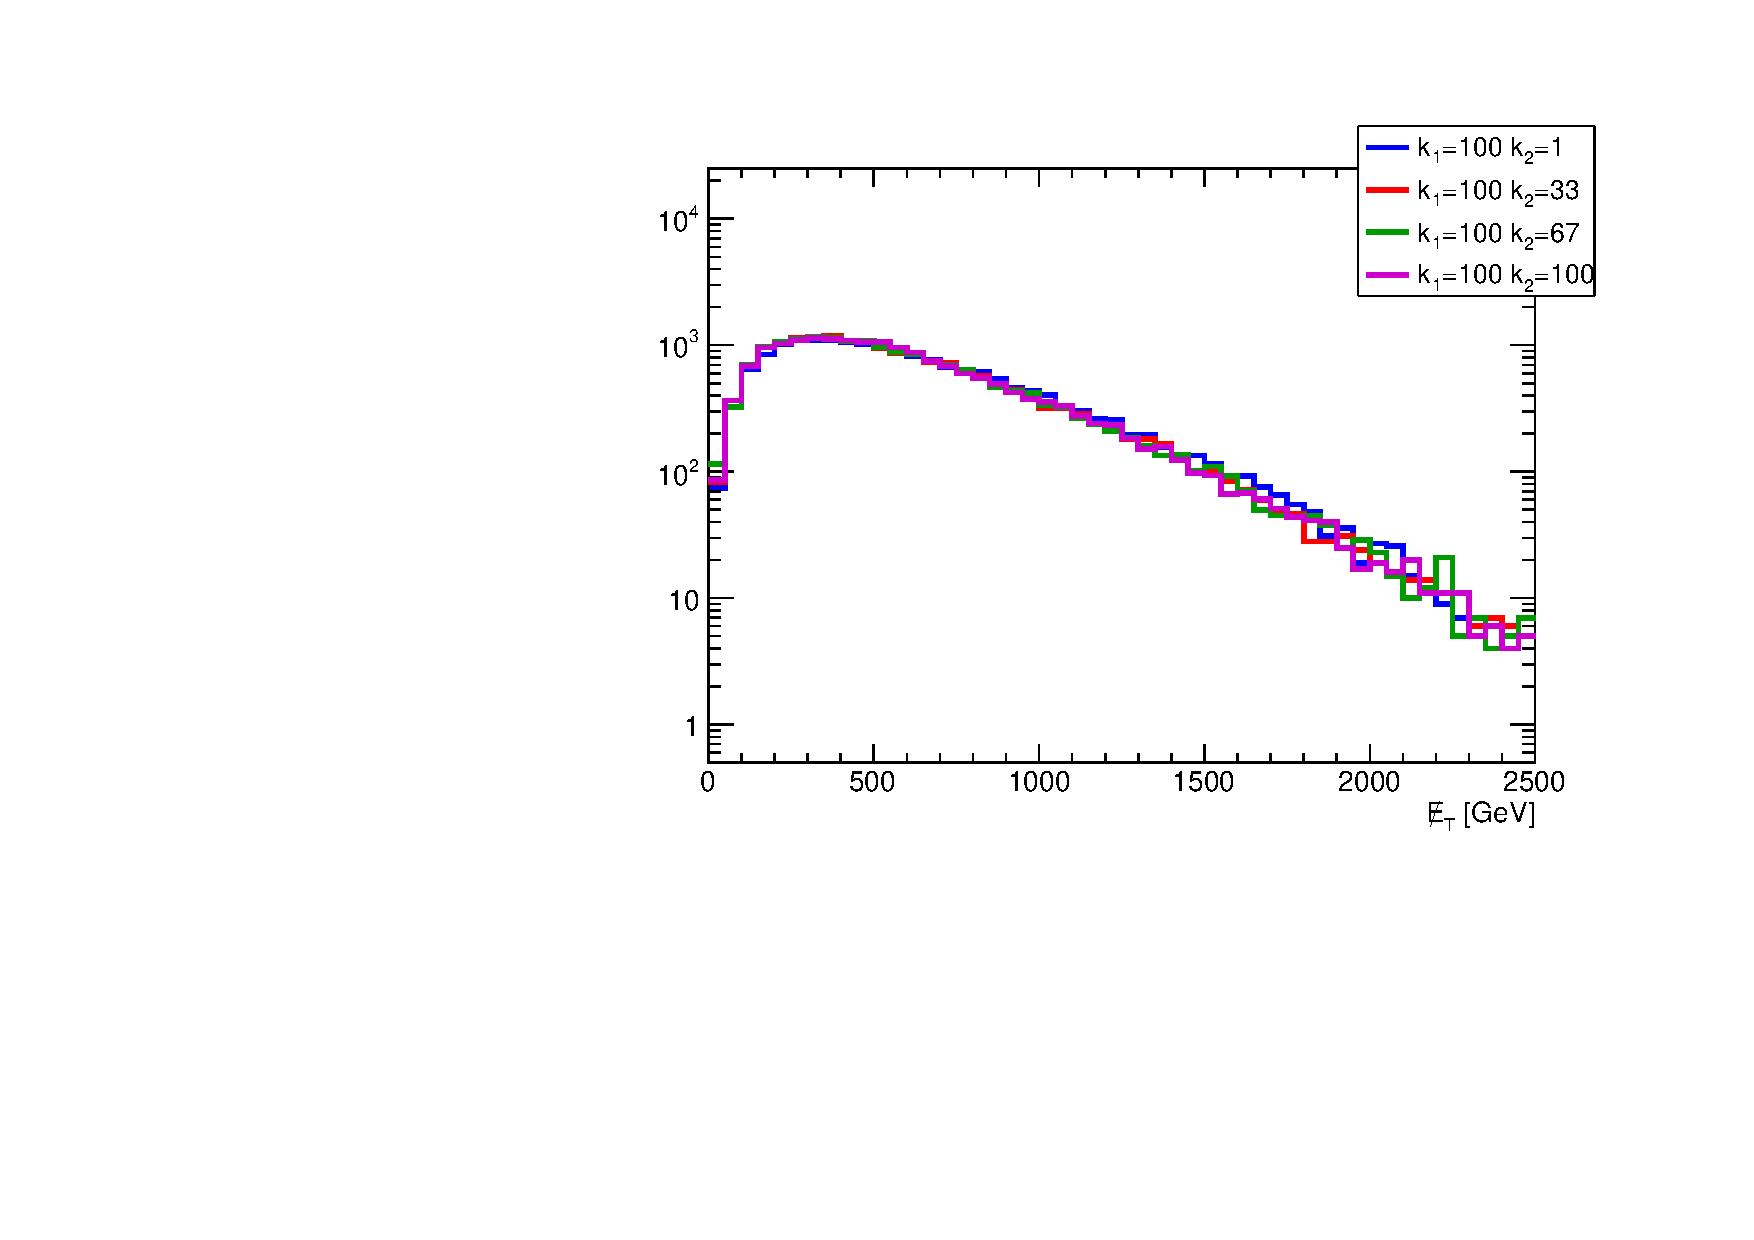
\includegraphics[width=0.95\textwidth]{figures/EW/monoZhad_SP/metPt}
%  }
%  \hfill
%  \subfloat[Acceptance.\label{fig:EFTD7_EW_Z_acc}]{%
%  	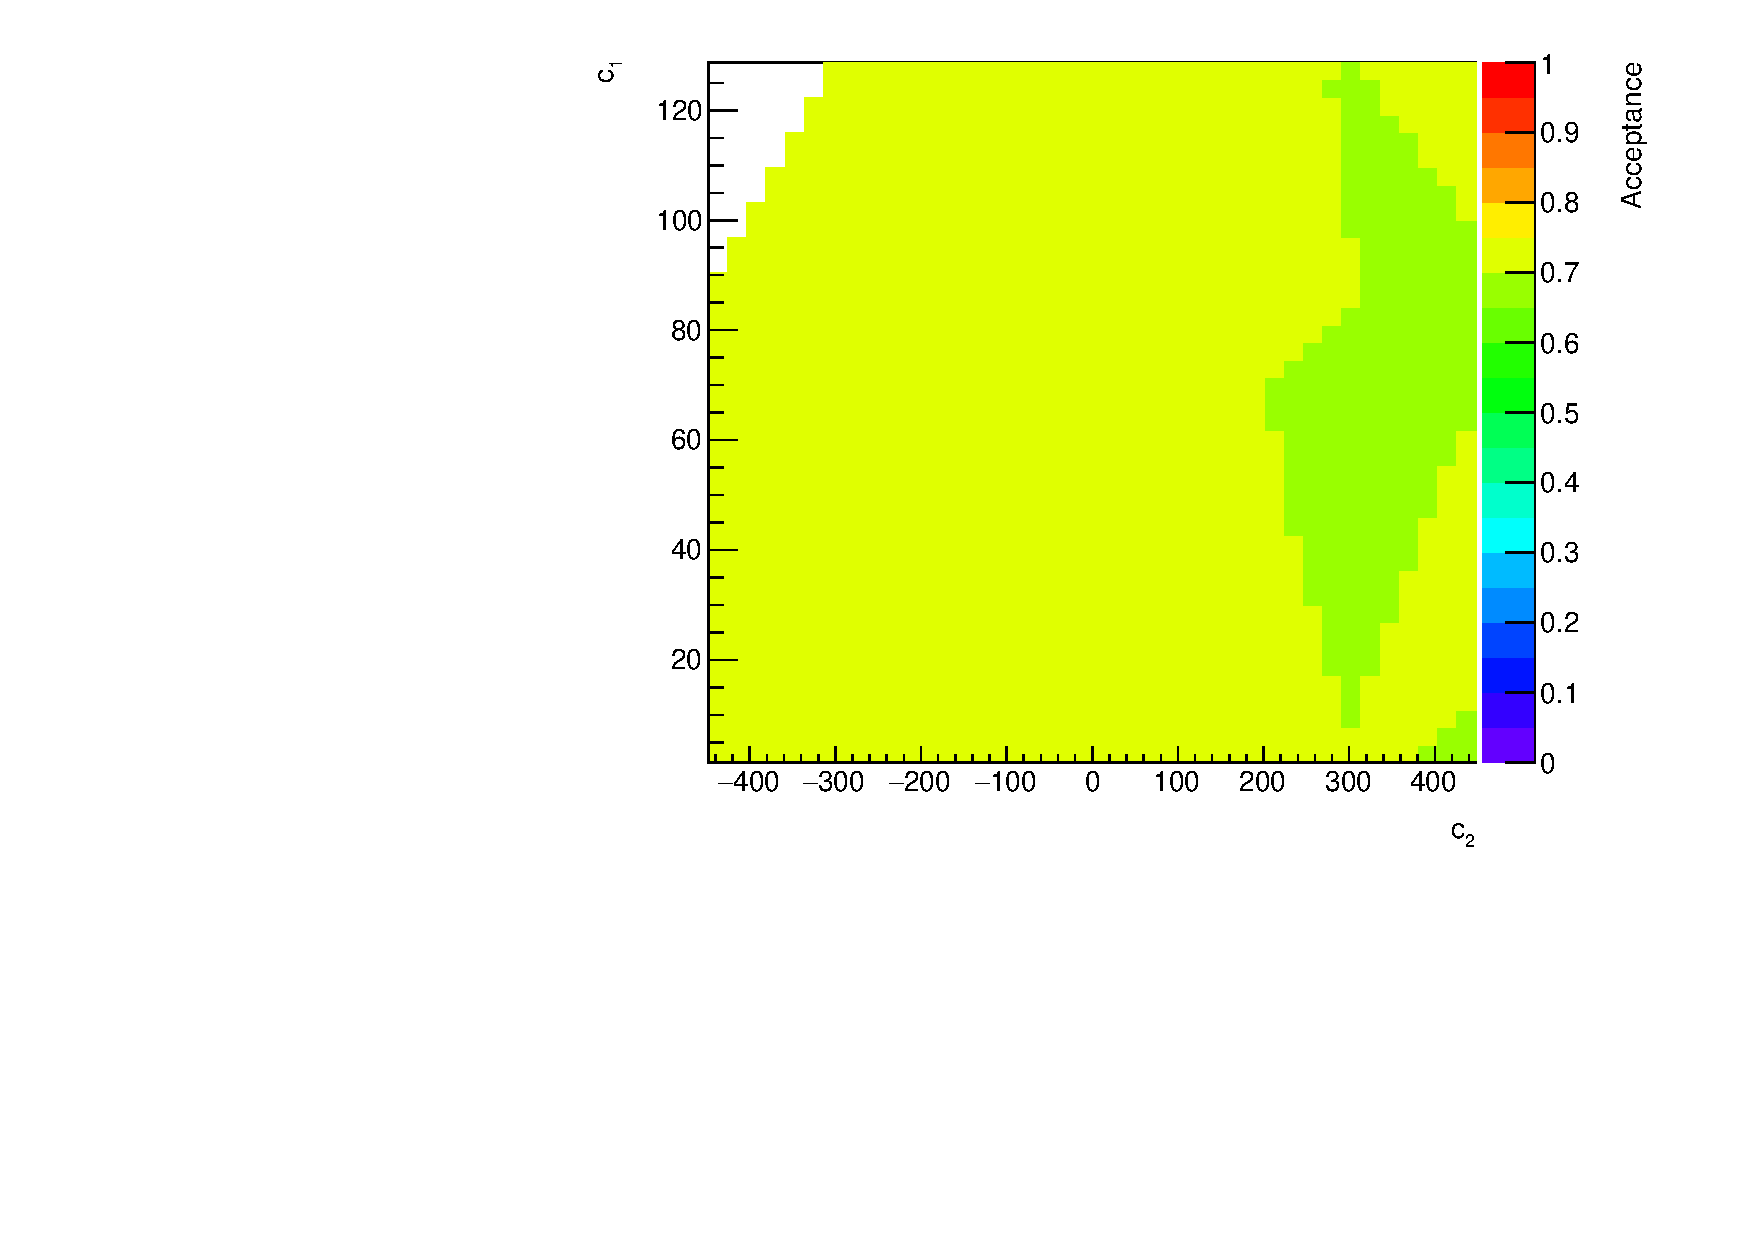
\includegraphics[width=0.7\textwidth]{figures/EW/monoZhad_SP/Sscale_newplot.pdf}
%  }
    \caption{\MET distribution for the dimension-7 model with a hadronically decaying Z in the final state,
    for the scalar and pseudoscalar operators representing direct interactions between DM and bosons. The values of the coefficients in the legend are multiplied by 100.}
    \label{fig:EFTD7_EW_kinematics}
\end{figure}


%%%%%%%%%%%%%Dimension 8 operators

\subsection{Higher dimensional operators}

Many higher dimensional operators can induce signals of photons or $W/Z/H$ bosons
in the final state. A complete list can be found in Refs.~\cite{Carpenter:2013xra, Berlin:2014cfa, Petrov:2013nia}
and references therein. 

Although with lower priority with respect to the operators above, 
a representative dimension-8 operators can be chosen as benchmark, with the form:
 
$$\frac{1}{\Lambda^4} \bar{\chiDM} \gamma^{\mu} \chiDM B_{\mu \nu} H^{\dagger} D^{\nu} H$$

In this case, the new physics scale is $\Lambda$ is connected with the coupling
of the DM as $\displaystyle y_{\chiDM} = \frac{1}{\Lambda^{4}}$.\Todo{Is more detail needed here?}
An advantage of this operator is that it includes all signatures with EW bosons,
allowing to assess the relative sensitivity of the various channels with the same model.  
The kinematics for this operator is different with respect to other operators,
leading to a harder \MET spectrum, 
as illustrated by comparing the leading $b-$jet distribution for the dimension 5 operator
to the dimension 8 operator. 
  
   \begin{figure}[hbpt!]
   	\centering
   	\subfloat[Dimension 5 operator]{
   		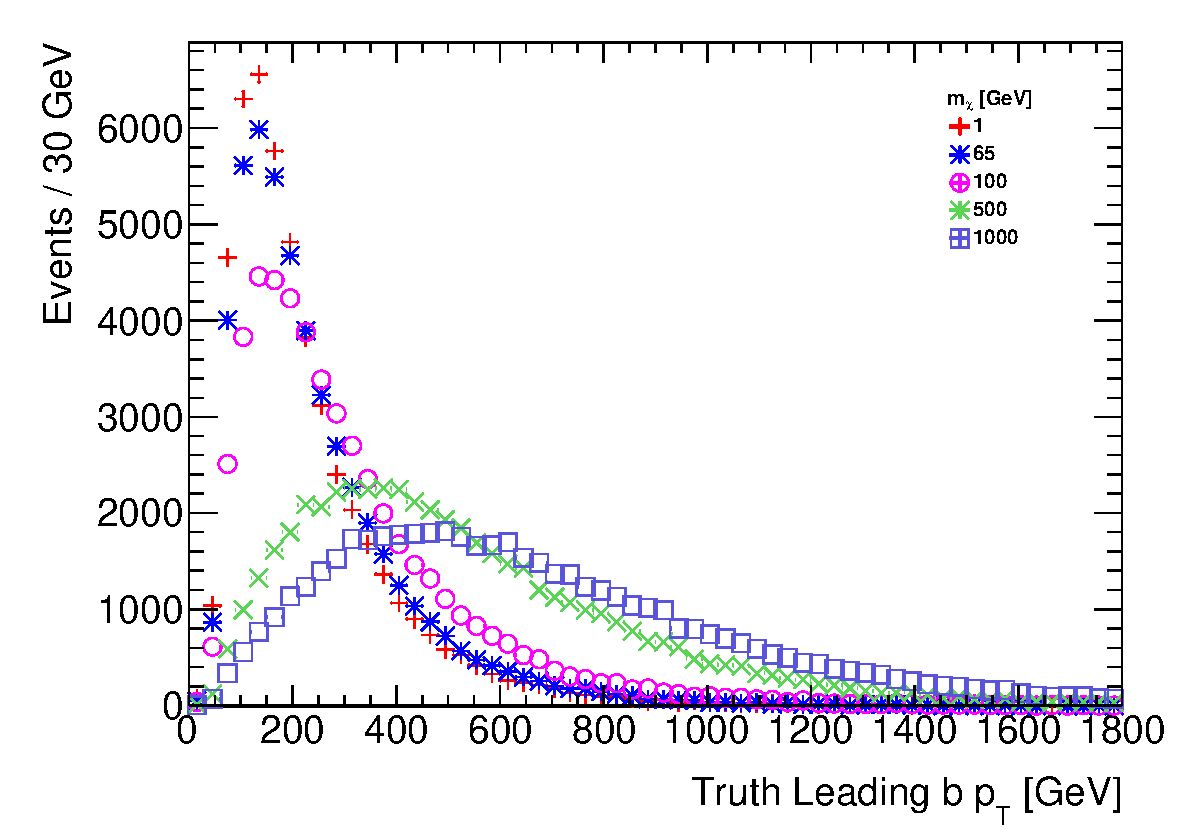
\includegraphics[width=0.95\linewidth]{figures/EW/monoH/xxhhg5/truth_leading_b_pt} %\label{fig:met_cmp_high}
   	}
   	\hfill
   	\subfloat[Dimension 7 operator]{
   		\includegraphics[width=0.95\linewidth]{figures/EW/monoH/xgxFhDh/truth_leading_b_pt} %\label{fig:met_cmp_high}
   	}
   	\caption{Comparison of the transverse momentum for the leading $b-$ jet from the Higgs decay for a dimension 5 and dimension 7 operator
   		with direct boson-DM couplings.}
   	\end{figure}
  

%\subsection{xgxFhDh Truth Kinematics}
%
%\begin{figure}[!htbp]
%	\begin{minipage}{0.5\textwidth}
%		\centering
%		\includegraphics[width = \linewidth]{xgxFhDh/truth_leading_b_pt.eps}
%	\end{minipage}
%	\begin{minipage}{0.5\textwidth}
%		\centering
%		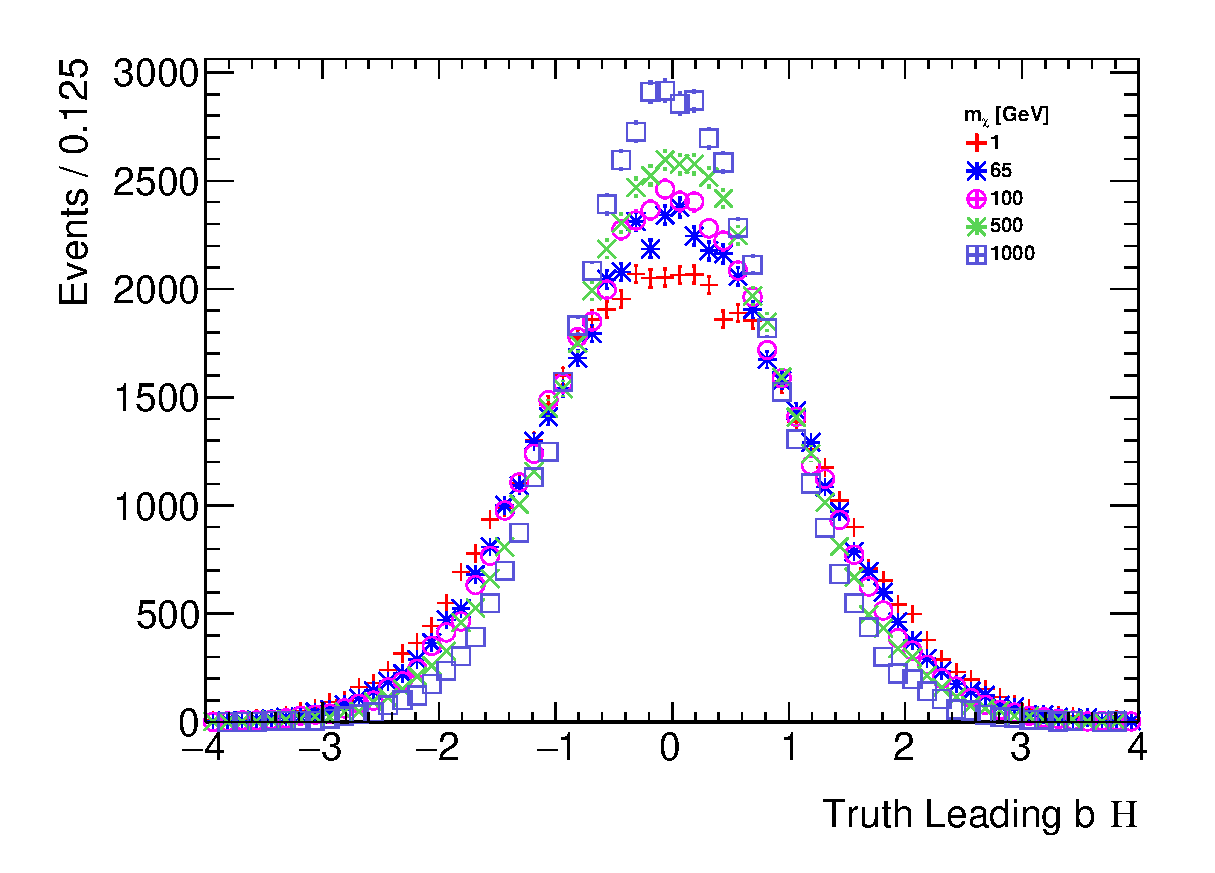
\includegraphics[width = \linewidth]{xgxFhDh/truth_leading_b_eta.eps}
%	\end{minipage}
%\end{figure}
%
%\begin{figure}[!htbp]
%	\begin{minipage}{0.5\textwidth}
%		\centering
%		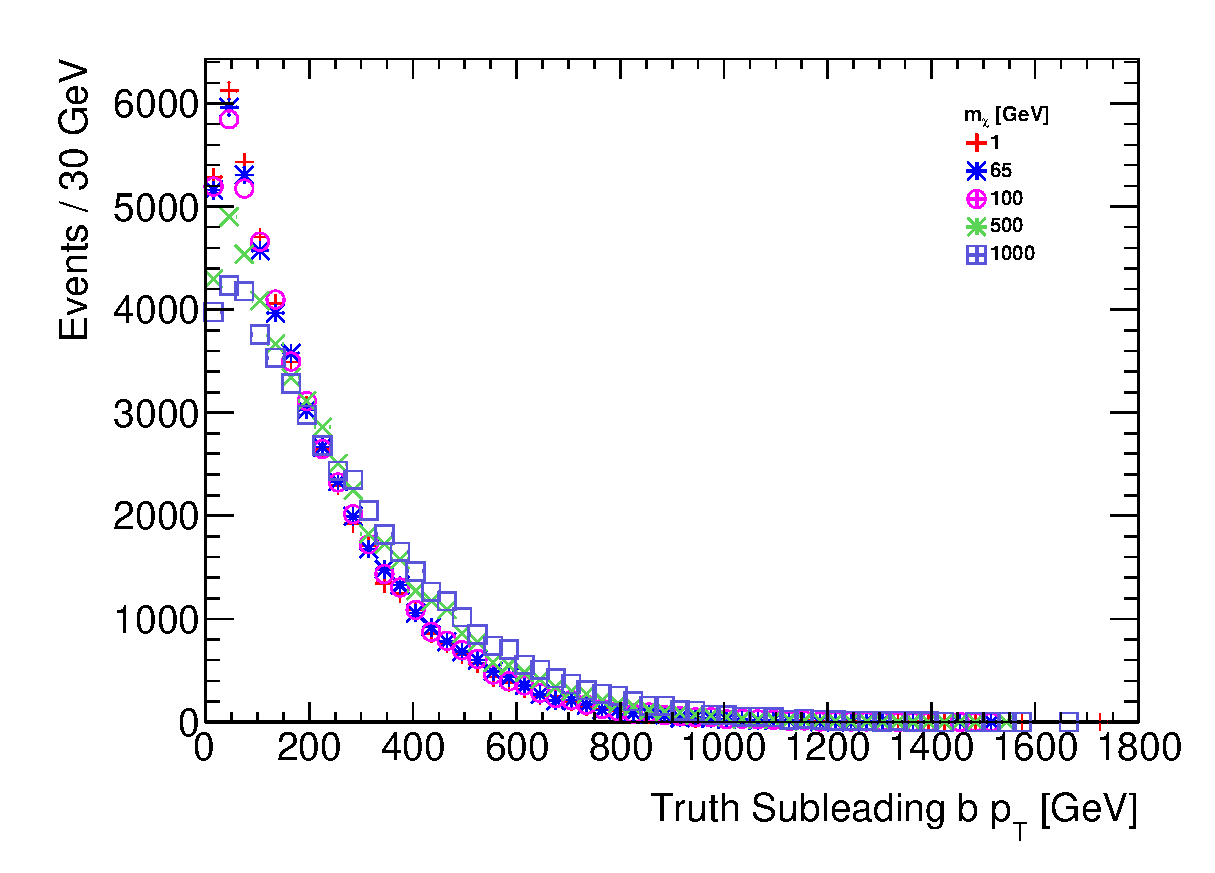
\includegraphics[width = \linewidth]{xgxFhDh/truth_subleading_b_pt.eps}
%	\end{minipage}
%	\begin{minipage}{0.5\textwidth}
%		\centering
%		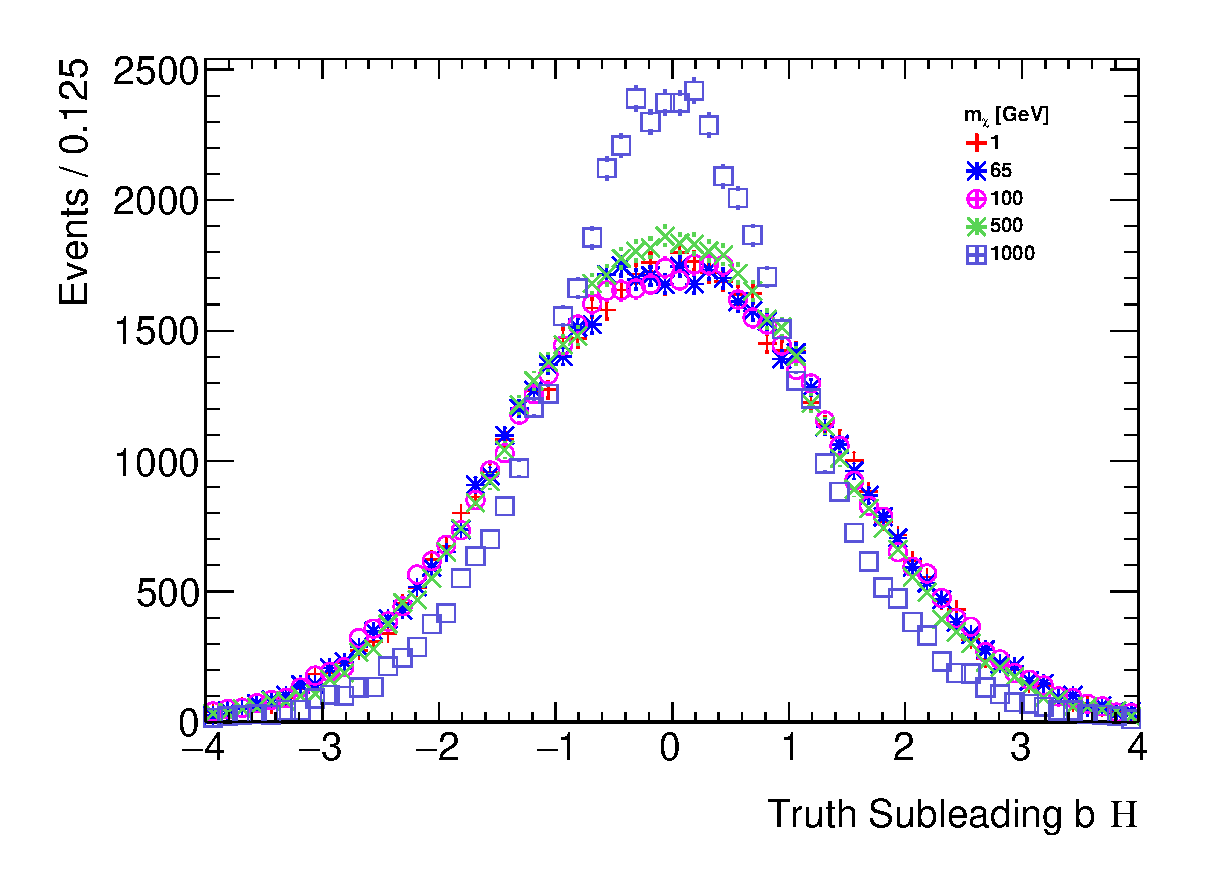
\includegraphics[width = \linewidth]{xgxFhDh/truth_subleading_b_eta.eps}
%	\end{minipage}
%\end{figure}
%
%\begin{figure}[!htbp]
%	\begin{minipage}{0.5\textwidth}
%		\centering
%		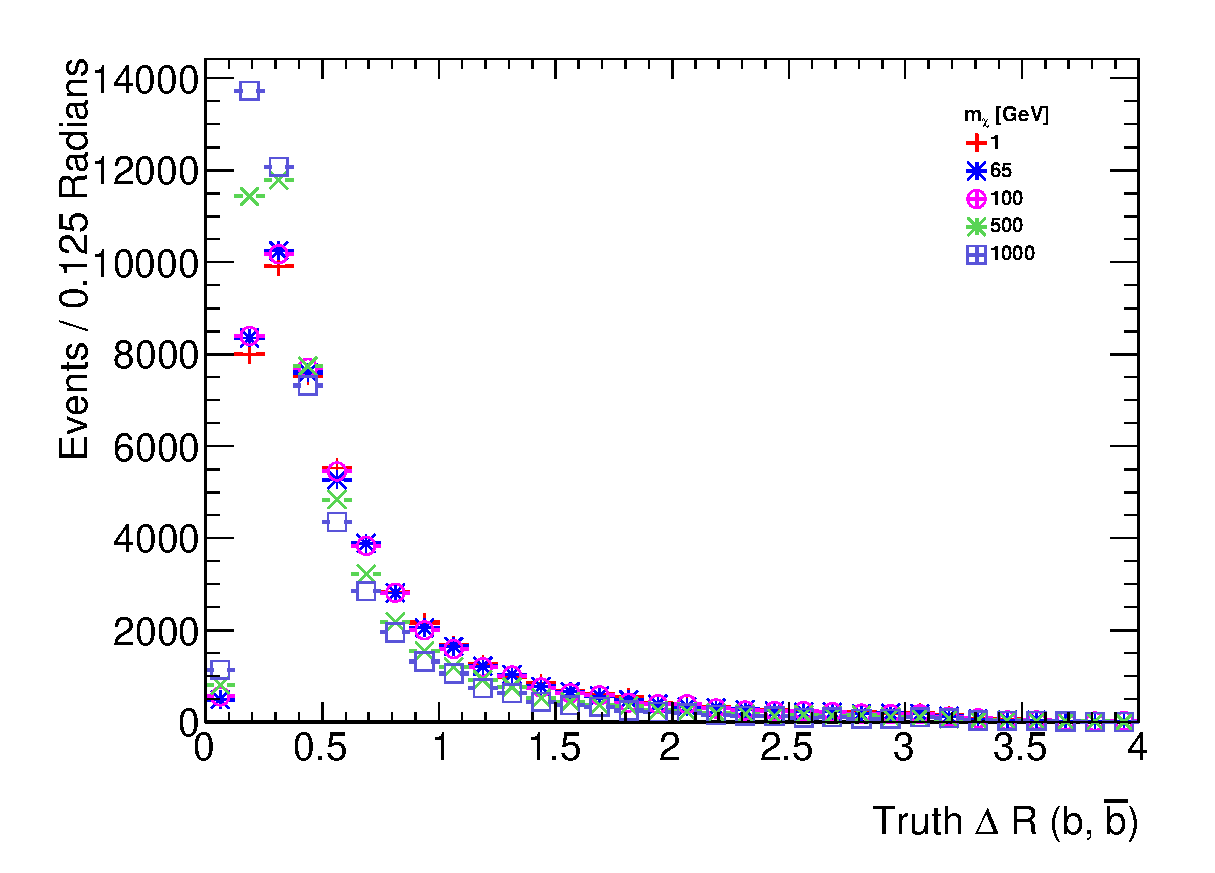
\includegraphics[width = \linewidth]{xgxFhDh/truth_bb_deltar.eps}
%	\end{minipage}
%\end{figure}
%
%\FloatBarrier
%\clearpage


\subsection{Validity of EW contact operators and possible completions}
\label{sub:validityEWContact}

It is important to remember that the operators described in 
this section may present problems in terms of the validity of the contact interaction
approach for the energy scales reached at the LHC. 

As outlined in~\cite{Berlin:2014cfa}, designing very high \MET search signal regions
that are exclusively motivated by the hard \MET spectra of the dimension 7 and 8 operators
will mean that the momentum transfer in the selected events is larger. This in turn
means that processes at that energy scale (mediators, particles exchanged in loops)
are accessible, and a simple contact interaction will not be able to correctly
describe the kinematics of these signals. 

Contact interaction operators like the ones in this section 
remain useful tools for comparison of the sensitivity of different search channels, 
and for reinterpretation of other models under the correct assumptions. 
To date, while UV-complete models are known, their phenomenology has
not been studied in full detail as their completion involves loops~\sidenote{
An example case for the need of loop completions is a simplified model with an additional scalar exchanged at tree level.
The scalar couples to $WW$ and $ZZ$ in a gauge-invariant way, Integrating out the mediator 
does not lead to the Lorentz structure of a dimension-7 operator, so it is not possible
to generate dimension-7 operators that satisfy gauge and Lorentz invariance at the same time.
A model with a \spinone mediator cannot be considered as an candidate for completion either, since dimension-7 operators only have scalar or pseudoscalar couplings.}. 

However, this may be the focus of future theoretical exploration, as discussed in Ref.~\cite{Crivellin:2015wva}.
An example of a complete model 
for scalar DM corresponding to the dimension-5 operator 
is provided in the Appendix~\ref{app:EWSpecificModels_Appendix}.
Providing results for the pure EFT limit of these models will prove useful
to cross-check the implementation of future. 

Given these considerations, we recommend to present results 
for these models as follows: 

\begin{itemize}
\item Deliver fiducial limits on the cross section of any new physics events, without any model assumption, according to the guidelines in Appendix~\ref{app:Presentation_Of_Experimental_Results}.  
\item Assess the percentage of events that pass a condition of validity for the EFT approximation that does not
depend on a specific completion, and present results removing 
of the invalid events using the procedure in Section~\ref{sec:EFTValidity} alongside the raw EFT results.
\end{itemize}


